\chapter*{Preliminary Concepts}
\section{Interpretable Sequential Decision Making}
\subsection{What is Sequential Decision Making?}
\begin{figure}[htbp]
    \centering
    \begin{tikzpicture}[
        node distance=2.5cm,
        auto,
        thick,
        state/.style={circle, draw, fill=blue!20, minimum size=1.5cm, text centered},
        environment/.style={rectangle, draw, dashed, fill=blue!10, rounded corners, minimum width=4cm, minimum height=2cm, text centered},
        agent/.style={rectangle, draw, fill=orange!20, rounded corners, minimum width=2cm, minimum height=1.5cm, text centered},
        robot/.style={rectangle, draw, fill=green!20, rounded corners, minimum width=2cm, minimum height=1.5cm, text centered},
        decision_box/.style={rectangle, draw, dashed, fill=gray!10, minimum width=7.5cm, minimum height=3cm, text centered},
        arrow/.style={->, thick, bend left=15},
        arrow_decision/.style={->, dashed, bend left=15}
    ]
        
        % Decision Making Box
        \node[decision_box] (decision_box) at (0.3,3.4) {};
        \node at (0.3,4.5) {\small{Decision Making}};
        
        % Robot (AI)
        \node[robot] (robot) at (-2.1,3.2) {
            \begin{minipage}{1.5cm}
                \centering
                \includesvg[width=0.4cm]{images/images_intro/robot-svgrepo-com.svg}\\
                \small{Computer program}
            \end{minipage}
        };
        
        % Doctor
        \node[agent] (doctor) at (2.5,3.2) {
            \begin{minipage}{1.5cm}
                \centering
                \includesvg[width=0.4cm]{images/images_intro/doctor-with-stethoscope-svgrepo-com.svg}\\
                \small{Doctor}
            \end{minipage}
        };
        
        % Environment (Patient)
        \node[environment] (environment) at (0,-0.5) {
            \begin{minipage}{2cm}
                \centering
                \includesvg[width=0.8cm]{images/images_intro/patient-4.svg}\\
                \small{Cancer patient}
            \end{minipage}
        };
        
        % Arrows
        \draw[arrow] (environment) to[bend left=30] node[left] {
            \begin{minipage}{2cm}
                \centering
                \includesvg[width=0.4cm]{images/images_intro/patient-clipboard-svgrepo-com.svg}\\
                \small{Updated health status}
            \end{minipage}
        } (robot);
        \draw[arrow_decision] (robot) to node[above] {\small{Recommends}} (doctor);
        \draw[arrow_decision] (doctor) to node[below] {\small{Interprets}} (robot);

        \draw[arrow] (doctor) to[bend left=30] node[right] {
            \begin{minipage}{1.5cm}
                \centering
                \includesvg[width=0.5cm]{images/images_intro/syringe-svgrepo-com.svg}\\
                \small{Administrate chemo}
            \end{minipage}
        } (environment);
        
    \end{tikzpicture}
    \caption{Sequential decision making in cancer treatment. The AI system reacts to the patient's current state (tumor size, blood counts, etc.) and makes a recommendation to the doctor, who administers the chemotherapy to the patient. The patient's state is then updated, and this cycle repeats over time.}
    \label{fig:cancer-treatment-sdm}
\end{figure}
In this manuscript we study algorithms for sequential decision making. Humans engage in sequential decision making in all aspects of life. In medicine, doctors have to decide how much chemotherapy to administrate based on the patient's current health in order to cure~\cite{cancer}. In agriculture, agronomists have to decide when to fertilize next based on the current soil and weather conditions in order to maximize plant growth~\cite{agriculture}. 
In automotive, the auto-pilot system has to decide how to steer the wheel next based on lidar sensors in order to maintain a safe trajectory~\cite{driving}. 
Those sequential decision making processes exhibits key similarities: an agent takes actions based on some current information to achieve some goal.

As computer scientists, we ought to design computer programs~\cite{knuth63} that can help humans during those sequential decision making processes. 
For example, as depicted in Figure~\ref{fig:cancer-treatment-sdm}, a doctor could benefit from a program that would recommend the ``best'' treatment given the patient's state. 
Machine learning algorithms~\cite{turing} output such helpful programs.
For non-sequential decision making, when the doctor only takes one decision and does not need to react to the updated patient's health, e.g. making a diagnosis about cancer type, a program can be fitted to example data: given lots of patient records and the associated diagnoses, the program learns to make the same diagnosis a doctor would given the same patient record, this is \textit{supervised} learning~\cite{sl}. 
In the cancer treatment example, the doctor follows its patient through time and adapts its treatment to the changing health of the patient. In that case, machine learning, and in particular, \textit{reinforcement} learning~\cite{sutton}, can be used to teach the program how take decisions that lead to the patient recovery in the future based on how the patient's health changes from one chemo dose to another.  
Such machine learning algorithms train more and more performing program that make their way into our society to, e.g. identify digits on images~\cite{lenet}, control tokamak fusion~\cite{tokamak}, or write the abstract of a scientific article~\cite{bert}.

However, the key problematic behind this manuscript is that those programs computations cannot be understood and verified by humans: the programs are black-box.
Next, we describe the notion of interpretability that is key to ensure safe deployment of computer programs trained with machine learning in critical sectors like medicine.

\subsection{What is Interpretability?}


Originally, the etymology of ``interpretability'' is the Latin ``interpretabilis'' meaning ``that can be understood and explained''.
According to the Oxford English dictionary, the first recorded use of the english word ``interpretability'' dates back to 1854 when the british logician George Boole (Figure~\ref{fig:george-boole}) described the addition of concepts:

\begin{displaycquote}[p.~48]{boole}
I would remark in the first place that the generality of a method in Logic
must very much depend upon the generality of its elementary processes and laws.
We have, for instance, in the previous sections of this work investigated, among
other things, the laws of that logical process of addition which is symbolized by
the sign +. Now those laws have been determined from the study of instances,
in all of which it has been a necessary condition, that the classes or things added
together in thought should be mutually exclusive. The expression x + y seems
indeed uninterpretable, unless it be assumed that the things represented by x
and the things represented by y are entirely separate; that they embrace no
individuals in common. And conditions analogous to this have been involved
in those acts of conception from the study of which the laws of the other
symbolical operations have been ascertained. The question then arises, whether
it is necessary to restrict the application of these symbolical laws and processes
by the same conditions of interpretability under which the knowledge of them
was obtained. If such restriction is necessary, it is manifest that no such thing
as a general method in Logic is possible. On the other hand, if such restriction
is unnecessary, in what light are we to contemplate processes which appear to
be uninterpretable in that sphere of thought which they are designed to aid?
\end{displaycquote}

\begin{figure}[htbp]
    \centering
    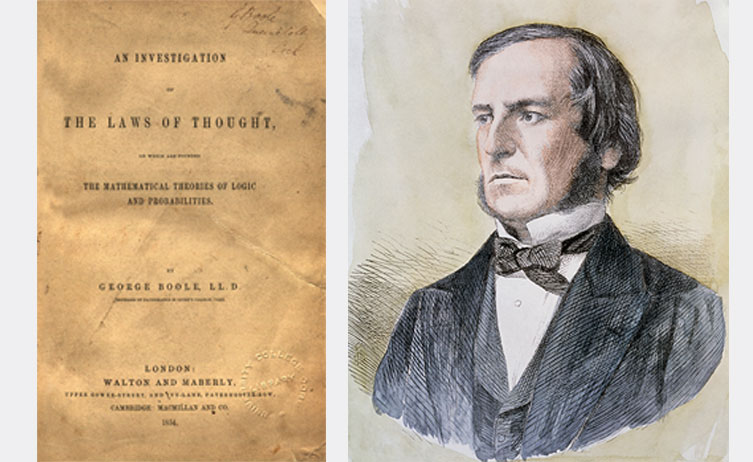
\includegraphics[width=0.5\textwidth]{images/images_intro/gboole.jpg}
    \caption{British logician and philosopher George Boole (1815-1864) next to its book \textit{The Laws of Thoughts} (1854) that is the oldest known record of the word ``interpretability''.}
    \label{fig:george-boole}
\end{figure}

What is remarkable is that the supposedly first recorded occurrence of ``interpretability'' was in the context of computer science. Boole asked: \textit{when can we meaningfully apply formal mathematical operations beyond the specific conditions under which we understand them?}
In Boole's era, the concern was whether logical operations like addition could be applied outside their original interpretable contexts—where symbols and their sum represent concepts that humans can understand, e.g. red + apples = red apples. Today, we face an analogous dilemma with machine learning algorithms: black-box programs like neural netowrks~\cite{perceptron}, that learn complex unintelligible combinations of inputs (representations), are often deployed in contexts where computations should be understood by humans, e.g., in medicine~\cite{black-box2}. 

\begin{figure}[htbp]
    \centering
    \begin{subfigure}[b]{0.7\textwidth}
        \centering
        \begin{tikzpicture}[
            node distance=2.5cm,
            auto,
            thick,
            state/.style={circle, draw, fill=blue!20, minimum size=1.5cm, text centered},
            environment/.style={rectangle, draw, dashed, fill=blue!10, rounded corners, minimum width=4cm, minimum height=2cm, text centered},
            agent/.style={rectangle, draw, fill=orange!20, rounded corners, minimum width=2cm, minimum height=1.5cm, text centered},
            robot/.style={rectangle, draw, fill=black!20, rounded corners, minimum width=2cm, minimum height=1.5cm, text centered},
            ml/.style={circle, draw, fill=purple!20, minimum width=2cm, minimum height=1cm, text centered},
            decision_box/.style={rectangle, draw, dashed, fill=gray!10, minimum width=7.5cm, minimum height=3cm, text centered},
            arrow/.style={->, thick, bend left=15},
            arrow_decision/.style={->, dashed, bend left=15}
        ]
            
            % Decision Making Box
            \node[decision_box] (decision_box) at (0.3,3.4) {};
            \node at (0.3,4.5) {\small{Decision Making}};
            
            % Robot (AI)
            \node[robot] (robot) at (-2.1,3.2) {
                \begin{minipage}{1.5cm}
                    \centering
                    \includesvg[width=0.4cm]{images/images_intro/network-mapping-svgrepo-com.svg}\\
                    \small{Neural network}
                \end{minipage}
            };
            
            % Doctor
            \node[agent] (doctor) at (2.5,3.2) {
                \begin{minipage}{1.5cm}
                    \centering
                    \includesvg[width=0.4cm]{images/images_intro/doctor-with-stethoscope-svgrepo-com.svg}\\
                    \small{Doctor}
                \end{minipage}
            };
            
            % Machine Learning component
            \node[ml] (ml) at (-7,3) {
                \begin{minipage}{1.8cm}
                    \centering
                    \includesvg[width=0.4cm]{images/images_intro/gear-file-svgrepo-com.svg}\\
                    \small{Machine learning}
                \end{minipage}
            };
            
            % Environment (Patient)
            \node[environment] (environment) at (0,-0.5) {
                \begin{minipage}{2cm}
                    \centering
                    \includesvg[width=0.8cm]{images/images_intro/patient-4.svg}\\
                    \small{Cancer patient}
                \end{minipage}
            };
            
            % Arrows
            \draw[arrow] (environment) to[bend left=30] node[left] {
                \begin{minipage}{2cm}
                    \centering
                    \includesvg[width=0.5cm]{images/images_intro/patient-clipboard-svgrepo-com.svg}\\
                    \small{Updated health status}
                \end{minipage}
            } (robot);
            \draw[arrow_decision] (robot) to node[above] {\small{Recommends}} (doctor);
            \draw[arrow_decision, red] (doctor) to node[below] {\small{Can't interpret}} (robot);
            
            \draw[arrow] (doctor) to[bend left=30] node[right] {
                \begin{minipage}{1.5cm}
                    \centering
                    \includesvg[width=0.5cm]{images/images_intro/syringe-svgrepo-com.svg}\\
                    \small{Administrate chemo}
                \end{minipage}
            } (environment);
            
            % ML learning arrows
            \draw[arrow] (environment) to[bend left=40] node[left] {
                \begin{minipage}{2cm}
                    \centering
                    \includesvg[width=0.5cm]{images/images_intro/patient-clipboard-svgrepo-com.svg}\\
                    \small{Treatment outcomes}
                \end{minipage}
            } (ml);
            \draw[arrow] (ml) to[bend left=20] node[above] {
                \begin{minipage}{1.5cm}
                    \centering
                    \small{Updates program}
                \end{minipage}
            } (robot);
            
        \end{tikzpicture}
        \caption{Black-box approach using neural networks}
        \label{fig:cancer-treatment-sdm-ml}
    \end{subfigure}
    
    \vspace*{1cm}
    
    \begin{subfigure}[b]{0.7\textwidth}
        \centering
        \begin{tikzpicture}[
            node distance=2.5cm,
            auto,
            thick,
            state/.style={circle, draw, fill=blue!20, minimum size=1.5cm, text centered},
            environment/.style={rectangle, draw, dashed, fill=blue!10, rounded corners, minimum width=4cm, minimum height=2cm, text centered},
            agent/.style={rectangle, draw, fill=orange!20, rounded corners, minimum width=2cm, minimum height=1.5cm, text centered},
            robot/.style={rectangle, draw, fill=green!20, rounded corners, minimum width=2cm, minimum height=1.5cm, text centered},
            ml/.style={circle, draw, fill=purple!20, minimum width=2cm, minimum height=1cm, text centered},
            decision_box/.style={rectangle, draw, dashed, fill=gray!10, minimum width=7.5cm, minimum height=3cm, text centered},
            arrow/.style={->, thick, bend left=15},
            arrow_decision/.style={->, dashed, bend left=15}
        ]
            
            % Decision Making Box
            \node[decision_box] (decision_box) at (0.3,3.4) {};
            \node at (0.3,4.5) {\small{Decision Making}};
            
            % Robot (AI)
            \node[robot] (robot) at (-2.1,3.2) {
                \begin{minipage}{1.5cm}
                    \centering
                    \includesvg[width=0.4cm]{images/images_intro/decision-tree-svgrepo-com.svg}\\
                    \small{Decision tree}
                \end{minipage}
            };
            
            % Doctor
            \node[agent] (doctor) at (2.5,3.2) {
                \begin{minipage}{1.5cm}
                    \centering
                    \includesvg[width=0.4cm]{images/images_intro/doctor-with-stethoscope-svgrepo-com.svg}\\
                    \small{Doctor}
                \end{minipage}
            };
            
            % Machine Learning component
            \node[ml] (ml) at (-7,3) {
                \begin{minipage}{1.8cm}
                    \centering
                    \includesvg[width=0.4cm]{images/images_intro/gear-file-svgrepo-com.svg}\\
                    \small{Interpretable machine learning}
                \end{minipage}
            };
            
            % Environment (Patient)
            \node[environment] (environment) at (0,-0.5) {
                \begin{minipage}{2cm}
                    \centering
                    \includesvg[width=0.8cm]{images/images_intro/patient-4.svg}\\
                    \small{Cancer patient}
                \end{minipage}
            };
            
            % Arrows
            \draw[arrow] (environment) to[bend left=30] node[left] {
                \begin{minipage}{2cm}
                    \centering
                    \includesvg[width=0.5cm]{images/images_intro/patient-clipboard-svgrepo-com.svg}\\
                    \small{Updated health status}
                \end{minipage}
            } (robot);
            \draw[arrow_decision] (robot) to node[above] {\small{Recommends}} (doctor);
            \draw[arrow_decision, green] (doctor) to node[below] {\small{Can interpret}} (robot);
            
            \draw[arrow] (doctor) to[bend left=30] node[right] {
                \begin{minipage}{1.5cm}
                    \centering
                    \includesvg[width=0.5cm]{images/images_intro/syringe-svgrepo-com.svg}\\
                    \small{Administrate chemo}
                \end{minipage}
            } (environment);
            
            % ML learning arrows
            \draw[arrow] (environment) to[bend left=40] node[left] {
                \begin{minipage}{2cm}
                    \centering
                    \includesvg[width=0.5cm]{images/images_intro/patient-clipboard-svgrepo-com.svg}\\
                    \small{Treatment outcomes}
                \end{minipage}
            } (ml);
            \draw[arrow] (ml) to[bend left=20] node[above] {
                \begin{minipage}{1.5cm}
                    \centering
                    \small{Updates program}
                \end{minipage}
            } (robot);
            
        \end{tikzpicture}
        \caption{Interpretable approach using decision trees}
        \label{fig:cancer-treatment-comparison}
    \end{subfigure}
    \caption{Comparison of sequential decision making approaches in cancer treatment. Top: A black-box neural network approach where the doctor cannot interpret the AI's recommendations. Bottom: An interpretable decision tree approach where the doctor can understand and verify the AI's recommendations. Both systems learn from treatment outcomes to improve their recommendations over time.}
    \label{fig:cancer-treatment-comparison-combined}
\end{figure}

In Figure~\ref{fig:cancer-treatment-sdm-ml}, we illustrate how existing machine learning algorithms \textit{could} be used in principle to help with cancer treatment. In truth this should be prohibited without some kind of transparency in the program's recommendation: why did the program recommended such dosage?
In Figure~\ref{fig:cancer-treatment-comparison}, we illustrate how machine learning \textit{should} be used in practice. We would ideally want doctors to have access to computer programs that can recommend ``good'' treatments and which recommendations are interpretable. 

The key challenge of doing research in interpretability is the lack of formalism; there is no \textit{formal} definition of what is an interpretable computer program. Hence, unlike for performance objectives which have well-defined optimization objective, e.g. maximizing accuracy (supervised learning) or maximizing rewards over time (reinforcement learning), it is not clear how to design machine learning algorithms to maximize interpretability of programs. 
Despite this lack of formalism the necessity of deploying interpretable models has sparked many works that we present next.
\subsection{What are existing approaches for learning interpretable programs?}
\begin{figure}[htbp]
    \centering
    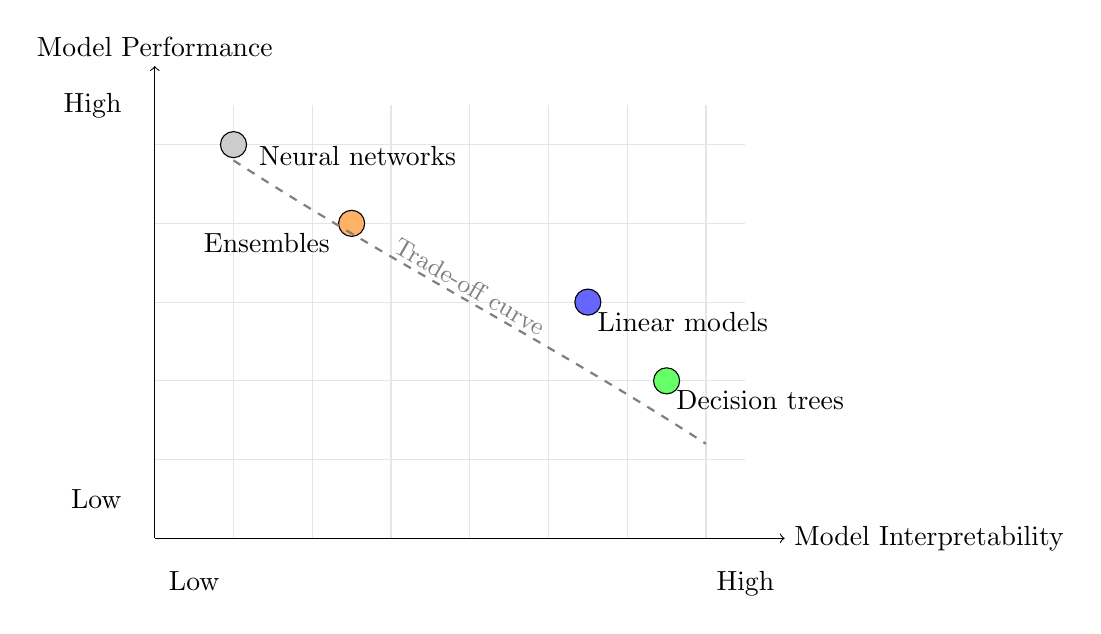
\begin{tikzpicture}
        % Define the axes
        \draw[->] (0,0) -- (8,0) node[right] {Model Interpretability};
        \draw[->] (0,0) -- (0,6) node[above] {Model Performance};
        
        % Add axis labels at the ends
        \node[below] at (0.5,-0.3) {Low};
        \node[below] at (7.5,-0.3) {High};
        \node[left] at (-0.3,0.5) {Low};
        \node[left] at (-0.3,5.5) {High};
        
        % Add grid lines (optional, subtle)
        \foreach \x in {1,2,...,7}
            \draw[gray!20] (\x,0) -- (\x,5.5);
        \foreach \y in {1,2,...,5}
            \draw[gray!20] (0,\y) -- (7.5,\y);
            
        % Position different model types
        % Deep Neural Networks (high performance, low interpretability)
        \node[circle, fill=black!20, draw, minimum size=8pt] at (1,5) {};
        \node[below right] at (1.2,5.1) {Neural networks};
        
        % Ensemble Methods (medium-high performance, low-medium interpretability)
        \node[circle, fill=orange!60, draw, minimum size=8pt] at (2.5,4) {};
        \node[below right] at (0.5,4) {Ensembles};
        
        % Linear Models (medium performance, high interpretability)
        \node[circle, fill=blue!60, draw, minimum size=8pt] at (5.5,3) {};
        \node[below right] at (5.5,3) {Linear models};
        
        % Decision Trees (medium-low performance, high interpretability)
        \node[circle, fill=green!60, draw, minimum size=8pt] at (6.5,2) {};
        \node[below right] at (6.5,2) {Decision trees};
        

        
        % Add a general trend line (optional)
        \draw[dashed, thick, gray] (1,4.8) .. controls (3,3.5) and (5,2.5) .. (7,1.2);
        \node[gray, rotate=-30] at (4,3.2) {\small Trade-off curve};
        
    \end{tikzpicture}
    \caption{The interpretability-performance trade-off in machine learning. Different program classes are positioned according to their typical interpretability and performance characteristics. The dashed line illustrates the general trade-off between these two properties.}
    \label{fig:interpretability-performance-tradeoff}
\end{figure}
Interpretable machine learning provides either local or global explanations \cite{glanois-survey}.
Global methods output a program which all recommendations can be interpreted without additional computations, e.g. a decision tree~\cite{breiman1984classification}. On the other hand, local methods require additional computations but are agnostic to the program class: they can give an \textit{approximate} interpretation of e.g. neural networks recommendations.
In Figure~\ref{fig:interpretability-performance-tradeoff} we present the popular trade-off between interpretability and performance of different program classes.

The most famous local explanation algorithm is LIME (Local Interpretable Model-agnostic Explanations)~\cite{lime}. Given a program class, LIME works by perturbing the input and learning a simple interpretable model locally to explain that particular prediction. For each individual prediction, LIME provides explanations by identifying which features were most important for that specific decision.
Hence, as stated above, LIME needs to learn a whole program per recommendation that needs to be interpreted; this is a lot of computations.
(Figure) HEATMAPS-FEATURE IMPORTANCE: key message is that Global => Local and Local =\=> Global.
\begin{figure}[htbp]
    \centering
    \begin{tikzpicture}[
        node distance=2cm,
        auto,
        thick,
        rl/.style={circle, draw, fill=purple!20, minimum width=1.5cm, minimum height=0.8cm, text centered},
        nn/.style={rectangle, draw, fill=black!20, rounded corners, minimum width=1.5cm, minimum height=1cm, text centered},
        sl/.style={circle, draw, fill=blue!20, minimum width=1.5cm, minimum height=0.8cm, text centered},
        dt/.style={rectangle, draw, fill=green!20, rounded corners, minimum width=1.5cm, minimum height=1cm, text centered},
        arrow/.style={->, thick},
        label/.style={font=\tiny, above},
        method_box/.style={rectangle, draw, dashed, minimum width=5cm, minimum height=3cm, text centered},
        method_box_indirect/.style={rectangle, draw, dashed, minimum width=9.5cm, minimum height=3cm, text centered}
    ]
        
        % Direct method box
        \node[method_box] (direct_box) at (-0.5,0) {};
        \node at (-0.5,1.7) {\small{Direct}};
        
        % Direct method - RL process
        \node[rl] (rl_direct) at (-2,0) {
            \begin{minipage}{1.2cm}
                \centering
                \includesvg[width=0.3cm]{images/images_intro/gear-file-svgrepo-com.svg}\\
                \tiny{Reinforcement learning}
            \end{minipage}
        };
        
        % Direct method - Decision Tree
        \node[dt] (dt_direct) at (1,0) {
            \begin{minipage}{1.2cm}
                \centering
                \includesvg[width=0.3cm]{images/images_intro/decision-tree-svgrepo-com.svg}\\
                \tiny{Decision tree}
            \end{minipage}
        };
        
        % Direct method arrow
        \draw[arrow] (rl_direct) -- (dt_direct) node[label, midway] {\tiny Learns};
        
        % Indirect method box
        \node[method_box_indirect] (indirect_box) at (7.1,0) {};
        \node at (6.8,1.7) {\small{Indirect}};
        
        % Indirect method - RL process
        \node[rl] (rl_indirect) at (3.5,0) {
            \begin{minipage}{1.2cm}
                \centering
                \includesvg[width=0.3cm]{images/images_intro/gear-file-svgrepo-com.svg}\\
                \tiny{Reinforcement learning}
            \end{minipage}
        };
        
        % Indirect method - Neural Network
        \node[nn] (nn_indirect) at (6,0) {
            \begin{minipage}{1.2cm}
                \centering
                \includesvg[width=0.3cm]{images/images_intro/network-mapping-svgrepo-com.svg}\\
                \tiny{Neural network}
            \end{minipage}
        };
        
        % Indirect method - Supervised Learning
        \node[sl] (sl_indirect) at (8.5,0) {
            \begin{minipage}{1.2cm}
                \centering
                \includesvg[width=0.3cm]{images/images_intro/gear-file-svgrepo-com.svg}\\
                \tiny{Supervised learning}
            \end{minipage}
        };
        
        % Indirect method - Decision Tree
        \node[dt] (dt_indirect) at (11,0) {
            \begin{minipage}{1.2cm}
                \centering
                \includesvg[width=0.3cm]{images/images_intro/decision-tree-svgrepo-com.svg}\\
                \tiny{Decision Tree}
            \end{minipage}
        };
        
        % Indirect method arrows
        \draw[arrow] (rl_indirect) -- (nn_indirect) node[label, midway] {\tiny Learns};
        \draw[arrow] (nn_indirect) -- (sl_indirect) node[label, midway] {\tiny Generates data};
        \draw[arrow] (sl_indirect) -- (dt_indirect) node[label, midway] {\tiny Learns};
        
    \end{tikzpicture}
    \caption{Comparison of direct and indirect approaches for learning interpretable policies in sequential decision making}
    \label{fig:direct-vs-indirect-methods}
\end{figure}

Global approaches are either direct or indirect~\cite{milani-survey}. 
Direct algorithms, such as decision tree induction~\cite{breiman1984classification}, are algorithms that directly search a space of interpretable programs (see Figure~\ref{fig:interpretability-performance-tradeoff}). One of the key challenges that motivates this thesis is that decision tree induction is only defined for supervised learning but not for reinforcement learning. It means that to directly learn computer programs for interpretable sequential decision making, one has to design completely new algorithms. 
What most existing research have focused on so far, is to work around this confinement of decision tree induction to supervised learning and develop indirect methods. 
Indirect methods for interpretable sequential decision making--sometimes called post-hoc--start with the reinforcement learning of a non-interpretable computer program, e.g., deep reinforcement learning of a neural network, and then use supervised learning of an interpretable model with the objective to emulate the non-interpretable program. This approach is called behavior cloning or imitation learning~\cite{behavior-cloning,dagger} and many, if not all, work on interpretable sequential decision making use this indirect approach\cite{viper,PIRL}.
Figure~\ref{fig:direct-vs-indirect-methods} illustrates the key difference between these two approaches. 

Researchers just recently started to study the advantage of direct over indirect learning of interpretable programs~\cite{topin2021iterative,leap}. In short, the motivation behind developing direct methods is to have the interpretable program optimized to solve your actual goal, e.g. patient treatment, while indirect methods learn an interpretable program that is optimized to match the behaviour of a non-interpretable model that was itself optimized to solve your goal. There is no guarantee that optimizing this indirect objective yields the ``best'' interpretability-performance trade-offs. 
Hence, the ideal solution to interpretable sequential decision making would be to have global direct algorithms.
\section{Other related works}
\subsection{Explainability}
\subsection{Misalignement}
\subsection{Programmatic RL}
\subsection{Causality}
\subsection{Mechanistic Interpretability in the era of large language models}
Next, we present the outline of this thesis.


\section{Outline of the Thesis}

In this thesis we take a stab at the difficult task of designing global direct algorithms for interpretable sequential decision making. In the first part of the manuscript we will present a mathematical formalism for the reinforcement learning of decision trees for sequential decision making. In particular we will show that indeed the direct approach can yield better trees than the indirect one. However the unfortunate key result from this opening part is that a good direct method cannot find decision trees for sequential decision making that are not \textit{very} easy.
Fortunately for us, in the second part of this manuscript, we show that some of these easy instances of interpretable sequential decision making tasks can be made \textit{non}-sequential giving rise to a whole new decision tree induction algorithm for supervised learning. In particular, we thoroughly benchmark our new decision tree induction algorithm and claim the state-of-the-art for decision tree induction.
Finally, after heavily studying decision trees and direct methods, we will leverage the diversity and simplicity of \textit{indirect} methods to compare other model classes of programs and show that in some cases neural networks can be considered more interpretable than trees and there exist problems for which there is no need to trade-off performance for interpretability. 
We summarize the outline of the manuscript in Figure~\ref{fig:thesis-outline} 

\begin{figure}[htbp]
    \centering
    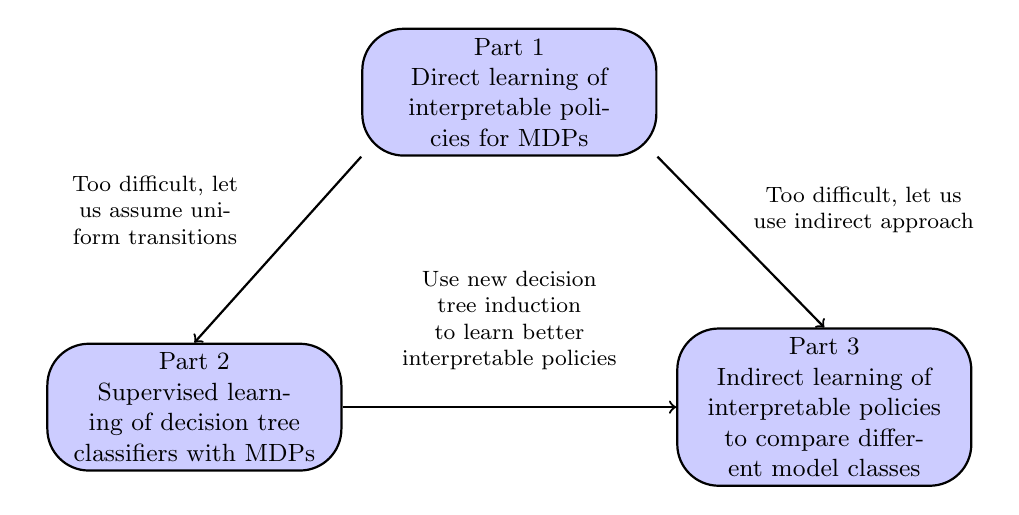
\begin{tikzpicture}[
        bubble/.style={rectangle, rounded corners=15pt, draw, thick, fill=blue!20, text width=3.5cm, text centered, minimum height=1.5cm, font=\small},
        arrow/.style={->, thick},
        label/.style={font=\footnotesize, text width=3cm, text centered}
    ]
        
        % Define the three vertices of the triangle
        % Top bubble - Chapter 1
        \node[bubble] (ch1) at (0,4) {Part 1\\Direct learning of interpretable policies for MDPs};
        
        % Bottom left bubble - Chapter 2  
        \node[bubble] (ch2) at (-4,0) {Part 2\\Supervised learning of decision tree classifiers with MDPs};
        
        % Bottom right bubble - Chapter 3
        \node[bubble] (ch3) at (4,0) {Part 3\\Indirect learning of interpretable policies to compare different model classes};
        
        % Arrow from Chapter 1 to Chapter 2
        \draw[arrow] (ch1.south west) -- (ch2.north);
        \node[label] at (-4.5,2.5) {Too difficult, let us assume uniform transitions};
        
        % Arrow from Chapter 1 to Chapter 3  
        \draw[arrow] (ch1.south east) -- (ch3.north);
        \node[label] at (4.5,2.5) {Too difficult, let us use indirect approach};

        % Arrow from Chapter 1 to Chapter 3  
        \draw[arrow] (ch2.east) -- (ch3.west);
        \node[label] at (0,1.1) {Use new decision tree induction to learn better interpretable policies};
        
        
    \end{tikzpicture}
    \caption{Thesis structure showing the progression from direct reinforcement learning of decision tree policies (Chapter 1) to simplified approaches: supervised learning with uniform transitions (Chapter 2) and indirect learning methods (Chapter 3).}
    \label{fig:thesis-outline}
\end{figure}



\section{Technical Preliminaries}
\subsection{What are decision trees?}
\begin{figure}[htbp]
    \centering
    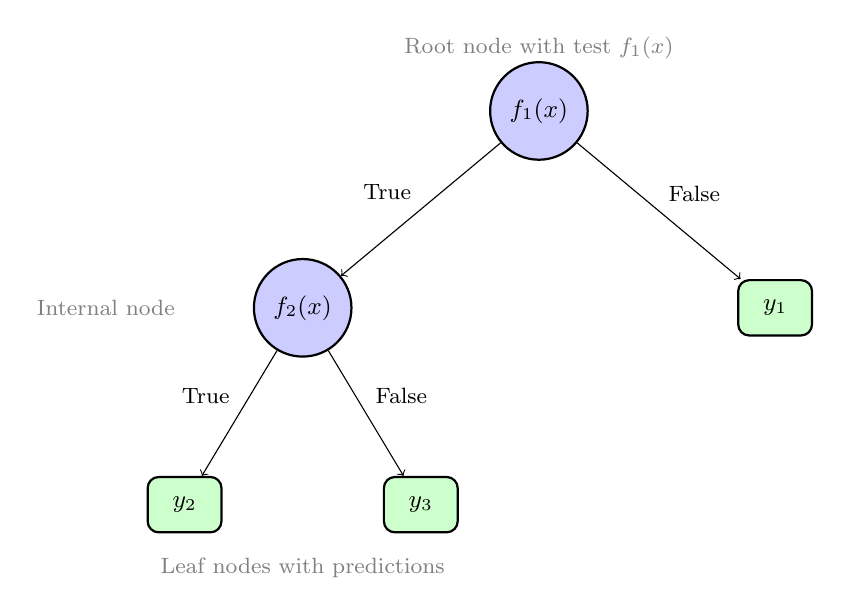
\begin{tikzpicture}[
        scale=1.0,
        decision/.style={circle, draw, thick, fill=blue!20, text width=2.5em, text centered, minimum height=2.5em, font=\small},
        leaf/.style={rectangle, draw, thick, fill=green!20, text width=2em, text centered, rounded corners, minimum height=2em, font=\small},
        edge_label/.style={font=\footnotesize, midway}
    ]
        % Root decision node
        \node[decision] (root) at (0,0) {$f_1(x)$};
        
        % Second level nodes
        \node[decision] (left_decision) at (-3, -2.5) {$f_2(x)$};
        \node[leaf] (right_leaf) at (3, -2.5) {$y_1$};
        
        % Third level nodes (leaves)
        \node[leaf] (left_left) at (-4.5, -5) {$y_2$};
        \node[leaf] (left_right) at (-1.5, -5) {$y_3$};
        
        % Connections with labels
        \draw[->] (root) -- (left_decision) node[edge_label, above left] {True};
        \draw[->] (root) -- (right_leaf) node[edge_label, above right] {False};
        \draw[->] (left_decision) -- (left_left) node[edge_label, above left] {True};
        \draw[->] (left_decision) -- (left_right) node[edge_label, above right] {False};
        
        % Add labels for components
        \node[font=\footnotesize, text=gray] at (0, 0.8) {Root node with test $f_1(x)$};
        \node[font=\footnotesize, text=gray] at (-5.5, -2.5) {Internal node};
        \node[font=\footnotesize, text=gray] at (-3, -5.8) {Leaf nodes with predictions};
        
    \end{tikzpicture}
    \caption{A generic decision tree structure. Internal nodes contain test functions $f_v(x): \mathcal{X} \rightarrow \{0,1\}$ that map input features to boolean values. Edges represent the outcomes of these tests (True/False), and leaf nodes contain predictions $y_\ell \in \mathcal{Y}$. For any input $x$, the tree defines a unique path from root to leaf.}
    \label{fig:decision-tree-structure}
\end{figure}
As mentioned earlier, as opposed to neural networks, decision trees are supposedly very interpretable because they only apply boolean operations on the program input without relying on internal complex representations.
\begin{definition}[Decision tree]
A decision tree is a rooted tree $T = (V, E)$ where:
\begin{itemize}
\item Each internal node $v \in V$ is associated with a test function $f_v: \mathcal{X} \rightarrow \{0, 1\}$ that maps input features $x \in \mathcal{X}$ to a boolean.
\item Each edge $e \in E$ from an internal node corresponds to an outcome of the associated test function.
\item Each leaf node $\ell \in V$ is associated with a prediction $y_\ell \in \mathcal{Y}$, where $\mathcal{Y}$ is the output space.
\item For any input $x \in \mathcal{X}$, the tree defines a unique path from root to leaf, determining the prediction $T(x) = y_\ell$ where $\ell$ is the reached leaf.
\end{itemize}
\end{definition}
\subsection{How to learn decision trees?}
\begin{figure}
    \centering
    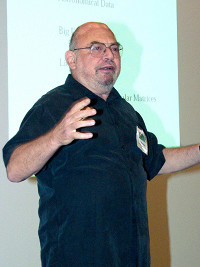
\includegraphics[width=0.3\textwidth]{images/images_intro/Leo_Breiman.jpg}
    \caption{The american statistician Leo Breiman (1928-2005) author of \textit{Classification and Regression Trees} (1984)}
    \label{fig:leo-breiman}
\end{figure}

The Classification and Regression Trees (CART) algorithm, developed by Leo Breiman and colleagues (Figure~\ref{fig:leo-breiman}), is one of the most widely used methods for learning decision trees from supervised data. CART builds binary decision trees through a greedy, top-down approach that recursively partitions the feature space. At each internal node, the algorithm selects the feature and threshold that best splits the data according to a purity criterion such as the Gini impurity for classification or mean squared error for regression.

CART uses threshold-based test functions of the form $f_v(x) = \mathbb{I}[x[feature] \leq threshold]$ where $\mathbb{I}[\cdot]$ is the indicator function, consistent with the general decision tree definition above. The key idea is to find splits that maximize the homogeneity of the resulting subsets. For classification, this means finding test functions that separate different classes as cleanly as possible. The algorithm continues splitting until a stopping criterion is met, such as reaching a minimum number of samples per leaf or achieving sufficient purity. The complete CART procedure is detailed in Algorithm~\ref{alg:cart}.


\RestyleAlgo{ruled}
\SetKwComment{Comment}{}{}
\begin{algorithm}
    \KwData{Training data $(X, y)$ where $X \in \mathbb{R}^{n \times d}$ and $y \in \{1, 2, \ldots, K\}^n$}
    \KwResult{Decision tree $T$}
    
    \SetKwProg{Fn}{Function}{:}{}
    \SetKwFunction{BuildTree}{BuildTree}
    \SetKwFunction{BestSplit}{BestSplit}
    \SetKwFunction{Gini}{Gini}
    \SetKwFunction{MajorityClass}{MajorityClass}
    
    \Fn{\BuildTree{$X, y$}}{
        \If{stopping criterion met}{
            \Return leaf node with prediction MajorityClass$(y)$
        }
        
        $(feature, threshold) \leftarrow$ BestSplit$(X, y)$ \\
        
        \If{no valid split found}{
            \Return leaf node with prediction MajorityClass$(y)$
        }
        
        Split data: $X_{left}, y_{left} = \{(x_i, y_i) : x_i[feature] \leq threshold\}$ \\
        \hspace{2.5cm} $X_{right}, y_{right} = \{(x_i, y_i) : x_i[feature] > threshold\}$ \\
        
        $left\_child \leftarrow$ BuildTree$(X_{left}, y_{left})$ \\
        $right\_child \leftarrow$ BuildTree$(X_{right}, y_{right})$ \\
        
        \Return internal node with test function $f_v(x) = \mathbb{I}[x[feature] \leq threshold]$ and children $(left\_child, right\_child)$
    }
    
    \Fn{\BestSplit{$X, y$}}{
        $best\_gain \leftarrow 0$ \\
        $best\_feature \leftarrow None$ \\
        $best\_threshold \leftarrow None$ \\
        
        \For{each feature $f \in \{1, 2, \ldots, d\}$}{
            \For{each unique value $v$ in $X[:, f]$}{
                $y_{left} \leftarrow \{y_i : X[i, f] \leq v\}$ \\
                $y_{right} \leftarrow \{y_i : X[i, f] > v\}$ \\
                
                $gain \leftarrow$ Gini$(y) - \frac{|y_{left}|}{|y|}$Gini$(y_{left}) - \frac{|y_{right}|}{|y|}$Gini$(y_{right})$ \\
                
                \If{$gain > best\_gain$}{
                    $best\_gain \leftarrow gain$ \\
                    $best\_feature \leftarrow f$ \\
                    $best\_threshold \leftarrow v$ \\
                }
            }
        }
        \Return $(best\_feature, best\_threshold)$
    }
    
    \Fn{\Gini{$y$}}{
        \Return $1 - \sum_{k=1}^K \left(\frac{|\{i : y_i = k\}|}{|y|}\right)^2$ \Comment{// Gini impurity}
    }
    
    \Return BuildTree$(X, y)$
    \caption{CART Algorithm for Decision Tree Learning}\label{alg:cart}
\end{algorithm}


\subsection{Markov decision processes/problems}
\begin{figure}[htbp]
    \centering
    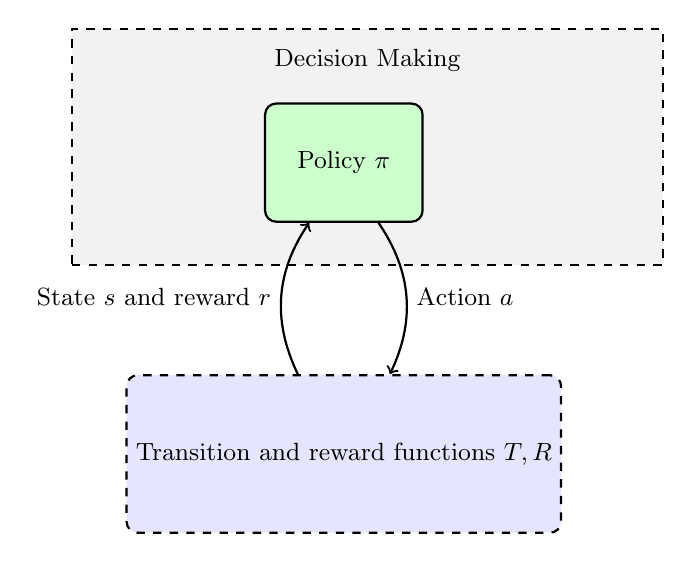
\begin{tikzpicture}[
        node distance=2.5cm,
        auto,
        thick,
        state/.style={circle, draw, fill=blue!20, minimum size=1.5cm, text centered},
        environment/.style={rectangle, draw, dashed, fill=blue!10, rounded corners, minimum width=4cm, minimum height=2cm, text centered},
        agent/.style={rectangle, draw, fill=orange!20, rounded corners, minimum width=2cm, minimum height=1.5cm, text centered},
        robot/.style={rectangle, draw, fill=green!20, rounded corners, minimum width=2cm, minimum height=1.5cm, text centered},
        decision_box/.style={rectangle, draw, dashed, fill=gray!10, minimum width=7.5cm, minimum height=3cm, text centered},
        arrow/.style={->, thick, bend left=15},
        arrow_decision/.style={->, dashed, bend left=15}
    ]
        
        % Decision Making Box
        \node[decision_box] (decision_box) at (0.3,3.4) {};
        \node at (0.3,4.5) {\small{Decision Making}};
        
        % Robot (AI)
        \node[robot] (robot) at (0,3.2) {\small{Policy $\pi$}};
        
        
        % Environment (Patient)
        \node[environment] (environment) at (0,-0.5) {\small{Transition and reward functions $T, R$}};
        
        % Arrows
        \draw[arrow] (environment) to[bend left=30] node[left] {\small{State $s$ and reward $r$}} (robot);
        \draw[arrow] (robot) to[bend left=30] node[right] {\small{Action $a$}} (environment);
        
    \end{tikzpicture}
    \caption{Markov decision process}
    \label{fig:MDP}
\end{figure}
Markov decision processes (MDPs) were first introduced in the 1950s by Richard Bellman (cite). Informally, an MDP models how an agent acts over time to achieve its goal. At every timestep, the agent observes its current state, e.g. a patient weight and tumor size, and takes an action, e.g. injects a certain amount of chemotherapy. When doing a certain action in a certain state, the agent gets a reward that helps it evaluate the quality of its action with respect to its goal, e.g., the tumor size decrease when the agent has to cure cancer. Finally, the agent is provided with a new state, e.g. the updated patient state, and repeats this process over time. Following Martin L. Puterman's book on MDPs (cite), we formally define as follows.
\begin{definition}[Markov decision process] An MDP is a tuple $\mathcal{M} = \langle S, A, R, T, T_0 \rangle$ where:
\begin{itemize}
\item $S$ is a finite set of states $s \in \mathbb{R}^n$ representing all possible configurations of the environment.
\item $A$ is a finite set of actions $a \in \mathbb{Z}^m$ available to the agent.
\item $R: S \times A \rightarrow \mathbb{R}$ is the reward function that assigns a real-valued reward to each state-action pair.
\item $T: S \times A \rightarrow \Delta(S)$ is the transition function that maps state-action pairs to probability distributions over next states, where $\Delta(S)$ denotes the probability simplex over $S$.
\item $T_0 \in \Delta(S)$ is the initial distribution over states.
\end{itemize}
\end{definition}
Now we can also model the ``goal'' of the agent. Informally, the goal of an agent is to behave such that it gets as much reward as it can over time. For example, in the cancer treatment case, the best reward the agent can get is to completely get rid of the patient's tumor after some time. Furthermore, we want our agent to prefer behaviour that gets rid of the patient's tumor as fast as possible. We can formally model the agent's goal as an optimization problem as follows. %talk about alignment?
\begin{definition}[Markov decision problem] Given an MDP $\mathcal{M}=\langle S, A, R, T, T_0 \rangle$, the goal of an agent following policy $\pi: S \rightarrow A$ is to maximize the expected discounted sum of rewards:
$$J(\pi) = \mathbb{E}\left[\sum_{t=0}^{\infty} \gamma^t R(s_t, a_t) \mid s_0 \sim T_0, a_t = \pi(s_t), s_{t+1} \sim T(s_t, a_t)\right]$$
where $\gamma \in (0,1)$ is the discount factor that controls the trade-off between immediate and future rewards.
\end{definition}

Hence, algorithms presented in this manuscript aim to find solutions to Markov decision problems, i.e. the optimal policy: $\pi^\star =\underset{\pi}{\operatorname{argmax}}J(\pi)$
For the rest of this text, we will use an abuse of notation and denote both a Markov decision process and the associated Markov decision problem by MDP.
\subsection{Exact solutions for Markov decision problems}
It is possible to compute the exact optimal policy $\pi^\star$ using dynamic programming (cite). Indeed, one can leverage the Markov property to find for all states the best action to take based on the reward of upcoming states.
\begin{definition}[Value of a state] The value of a state $s\in S$ under policy $\pi$ is the expected discounted sum of rewards starting from state $s$ and following policy $\pi$:
    $$V^\pi(s) = \mathbb{E}\left[\sum_{t=0}^{\infty} \gamma^t R(s_t, a_t) \mid s_0 = s, a_t = \pi(s_t), s_{t+1} \sim T(s_t, a_t)\right]$$
    Applying the Markov property gives a recursive definition of the value of $s$ under policy $\pi$:
    $$V^\pi(s) = R(s,\pi(s)) + \gamma \sum_{s' \in S} T^{s'}(s,\pi(s))V^\pi(s')$$
    where $T^{s'}(s,\pi(s))$ is the probability of transitioning to state $s'$ when taking action $\pi(s)$ in state $s$.
\end{definition}
\begin{definition}[Optimal value of a state] The optimal value of a state $s\in S$, $V^\star(s)$, is the value of state $s$ when following the optimal policy: $V^{\pi^{\star}}(s)$.
    $$V^{\star}(s) = V^{\pi^{\star}}(s) = \underset{\pi}{\max}\left[J(\pi)\right]$$
\end{definition}
\begin{definition}[Optimal value of a state-action pair] The optimal value of a state-action pair $(s,a)\in S\times A$, $Q^\star(s,a)$, is the value of state $s$ when taking action $a$ and then following the optimal policy: $V^{\pi^{\star}}(s)$.
    $$Q^{\star}(s,a) = Q^{\pi^{\star}}(s) = R(s, a) + \gamma\sum_{s'\in S}V^{\star}(s')$$
\end{definition}

Hence, the algorithms we study in the thesis can also be seen as solving the problem: $\pi^{\star} = \underset{\pi}{\operatorname{argmax}}\mathbb{E}\left[V^{\pi}(s_0)|s_0\sim T_0 \right]$. The well-known Value Iteration algorithm~\ref{alg:value_iteration} solves this problem exactly (cite). 

\RestyleAlgo{ruled}
\SetKwComment{Comment}{}{}
\begin{algorithm}
    \KwData{MDP $\mathcal{M} = \langle S, A, R, T, T_0 \rangle$, convergence threshold $\theta$}
    \KwResult{Optimal policy $\pi^*$}
    Initialize $V(s) = 0$ for all $s \in S$ \\
    \Repeat{$\Delta < \theta$}{
        $\Delta \leftarrow 0$ \\
        \For{each state $s \in S$}{
            $v \leftarrow V(s)$ \\
            $V(s) \leftarrow \max_a \left[ R(s,a) + \gamma \sum_{s' \in S} T(s,a,s') V(s') \right]$ \Comment{// Bellman optimality update}
            $\Delta \leftarrow \max(\Delta, |v - V(s)|)$
        }
    }
    \For{each state $s \in S$}{
        $\pi^*(s) \leftarrow \arg\max_a \left[ R(s,a) + \gamma \sum_{s' \in S} T(s,a,s') V(s') \right]$ \Comment{// Extract optimal policy}
    }
    \caption{Value Iteration}\label{alg:value_iteration}
\end{algorithm}

More realistically, neither the transition kernel $T$ nor the reward function $R$ of the MDP are known, e.g., the doctor can't \textbf{know} how the tumor and the patient health will change after a dose of chemotherapy, it can only \textbf{observe} the change. This distinction between the information available to the agent is paralleled with the distinction between dynamic programming and reinforcement learning (RL) that we describe next. 
\subsection{Reinforcement learning of approximate solutions to MDPs}
\begin{figure}
    \centering
    \begin{subfigure}[b]{0.22\textwidth}
        \centering
        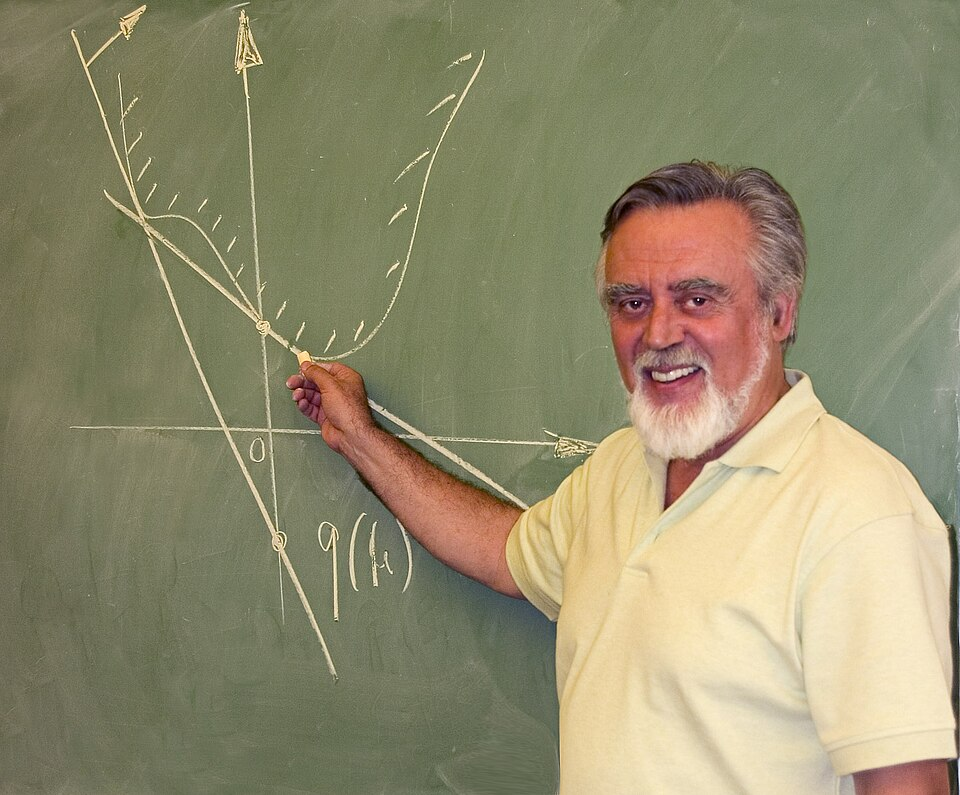
\includegraphics[width=\textwidth]{images/images_intro/Dimitri_Wiki_Pict.jpg}
        \caption{D. Bertsekas}
    \end{subfigure}
    \hfill
    \begin{subfigure}[b]{0.22\textwidth}
        \centering
        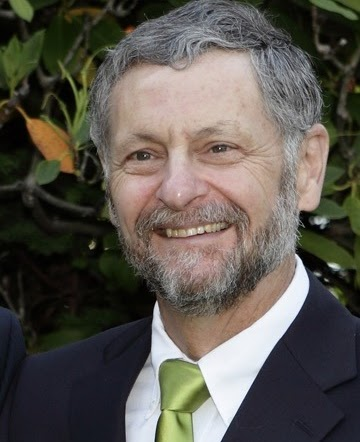
\includegraphics[width=0.7\textwidth]{images/images_intro/puterman.jpg}
        \caption{M.L. Puterman}
    \end{subfigure}
    \hfill
    \begin{subfigure}[b]{0.22\textwidth}
        \centering
        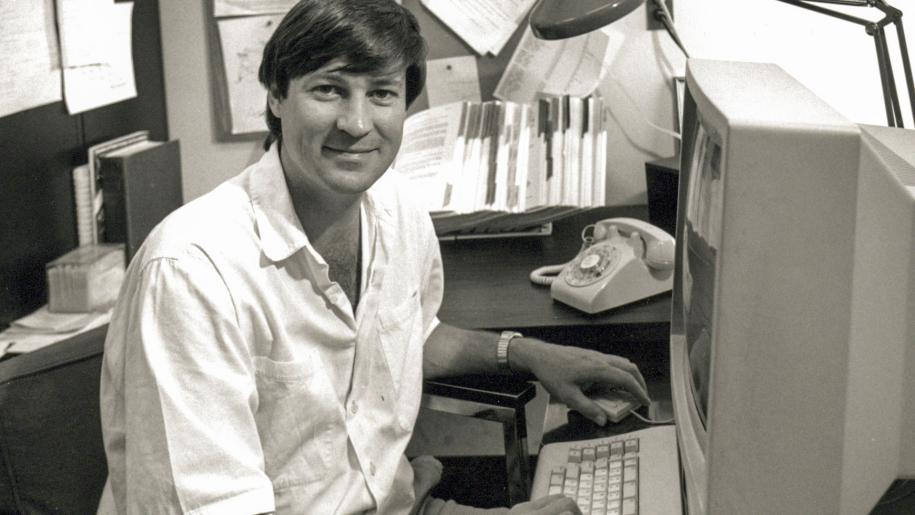
\includegraphics[width=1.2\textwidth]{images/images_intro/Barto_1982_umass_amherst.jpg}
        \caption{A. Barto}
    \end{subfigure}
    \hfill
    \begin{subfigure}[b]{0.22\textwidth}
        \centering
        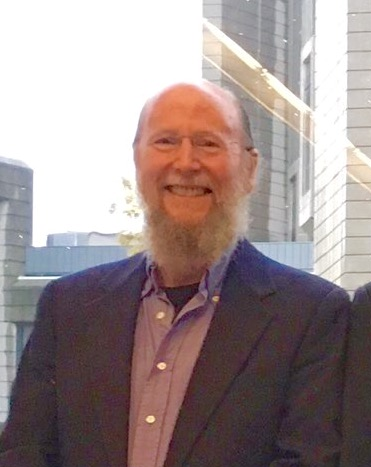
\includegraphics[width=0.67\textwidth]{images/images_intro/sutton.jpg}
        \caption{R. Sutton}
    \end{subfigure}
       \caption{The godfathers of sequential decision making. Andrew Barto and Richard Sutton are the ACM Turing Prize 2024 laureate and share an advisor advisee relationship.}
       \label{fig:rl-pioneers}
\end{figure}
Reinforcement learning algorithms popularized by Richard Sutton (Figure~\ref{fig:rl-pioneers}) (cite) don't \textbf{compute} an optimal policy but rather \textbf{learn} an approximate one based on sequences of observations ${(s_t, a_t, r_t, s_{t+1})}_t$.
RL algorithms usually fall into two categories: value-based (cite) and policy gradient (cite). The first group of RL algorithms computes an approximation of $V^{\star}$ using temporal difference learning, while the second class leverages the policy gradient theorem to approximate $\pi^{\star}$. Examples of these approaches are shown in Algorithms~\ref{alg:qlearning} and~\ref{alg:reinforce}.

\RestyleAlgo{ruled}
\SetKwComment{Comment}{}{}
\begin{algorithm}
    \KwData{MDP $\mathcal{M} = \langle S, A, R, T, T_0 \rangle$, learning rate $\alpha$, exploration rate $\epsilon$}
    \KwResult{Policy $\pi$}
    Initialize $Q(s,a) = 0$ for all $s \in S, a \in A$ \\
    \For{each episode}{
        Initialize state $s_0 \sim T_0$ \\
        \For{each step $t$}{
            Choose action $a_t$ using $\epsilon$-greedy: $a_t = \arg\max_a Q(s_t,a)$ with prob. $1-\epsilon$ \\
            Take action $a_t$, observe $r_t = R(s_t,a_t)$ and $s_{t+1} \sim T(s_t,a_t)$ \\
            $Q(s_t,a_t) \leftarrow Q(s_t,a_t) + \alpha[r_t + \gamma \max_{a'} Q(s_{t+1},a') - Q(s_t,a_t)]$ \\
            $s_t \leftarrow s_{t+1}$ \\
        }
    }
    $\pi(s) = \arg\max_a Q(s,a)$ \Comment{// Extract greedy policy}
    \caption{Value-based RL (Q-Learning)}\label{alg:qlearning}
\end{algorithm}

\RestyleAlgo{ruled}
\SetKwComment{Comment}{}{}
\begin{algorithm}
    \KwData{MDP $\mathcal{M} = \langle S, A, R, T, T_0 \rangle$, learning rate $\alpha$, policy parameters $\theta$}
    \KwResult{Policy $\pi_\theta$}
    Initialize policy parameters $\theta$ \\
    \For{each episode}{
        Generate trajectory $\tau = (s_0, a_0, r_0, s_1, a_1, r_1, \ldots)$ following $\pi_\theta$ \\
        \For{each timestep $t$ in trajectory}{
            $G_t \leftarrow \sum_{k=t}^{T} \gamma^{k-t} r_k$ \Comment{// Compute return}
            $\theta \leftarrow \theta + \alpha G_t \nabla_\theta \log \pi_\theta(a_t|s_t)$ \Comment{// Policy gradient update}
        }
    }
    \caption{Policy Gradient RL (REINFORCE)}\label{alg:reinforce}
\end{algorithm}

Both classes of algorithms are known to converge to the optimal value or policy under some conditions (cite) and have known great successes in real-world applications (cite).
The books from Puterman, Bertsekas, Sutton and Barto, offer a great overview of MDPs and algorithm to solve them.
There are many other ways to learn policies such as simple random search (cite) or model-based reinforcement learning. 
However, not many algorithms consider the learning of policies that can be easily understood by humans which we discuss next and that is the core of this manuscript.

\subsection{Imitation learning, the baseline (indirect) global interpretable reinforcement learning method}
\begin{algorithm}
    \caption{Imitate Expert~\cite{behavior-cloning,dagger,viper}}\label{alg:distill}
    \KwIn{Expert policy $\pi^*$, MDP $M$, policy class $\Pi$, number of iterations $N$, total samples $S$, importance sampling flag $I$}
    \KwOut{Fitted student policy $\hat{\pi}_i$}
    
    % Initialize empty dataset and initial policy
    Initialize dataset $\mathcal{D} \gets \emptyset$\;
    Initialize $\hat{\pi}_1$ arbitrarily from $\Pi$\;
    
    \For{$i \gets 1$ \KwTo $N$}{
        % Create mixed policy using expert and current policy
        \lIf{i = 1}{
        $\pi_i \gets \pi^*$\
        }
          \lElse{
            $\pi_i \gets \hat{\pi}_i$
          } \label{alg:expert-or-student}
        % Collect data using mixed policy
        Sample $S/N$ transitions from $M$ using $\pi_i$\;
        \lIf{$I$ is True}{
        $w(s) \gets V^{\pi*}(s) - \operatorname{min}_aQ^{\pi*}(s, a)$
        }
          \lElse{
            $w(s) \gets 1$
          }
        % Get expert actions for visited states
        Collect dataset $\mathcal{D}_i \gets \{ (s, \pi^*(s), w(s)) \}$ of states visited by $\pi_i$ and expert actions\;\label{alg:actions-expert}
        
        % Aggregate datasets
        $\mathcal{D} \gets \mathcal{D} \cup \mathcal{D}_i$\;
        
        % Train new policy
       Fit classifier/regressor $\hat{\pi}_{i+1}$ on $\mathcal{D}$\;\label{alg:fit}
    }
    
    \Return $\hat{\pi}_N$\;
    \end{algorithm}